% This file was created with tikzplotlib v0.10.1.
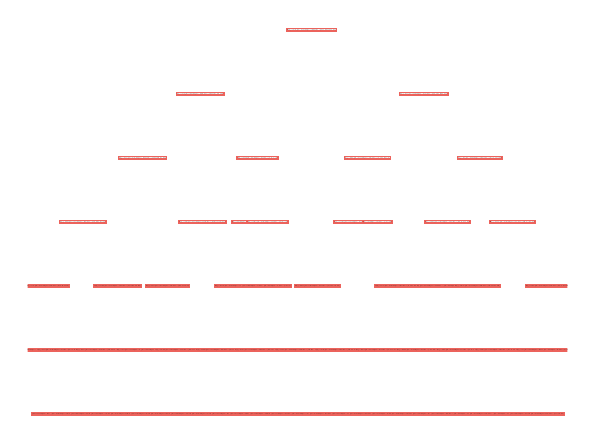
\begin{tikzpicture}

\definecolor{darkgray176}{RGB}{176,176,176}
\definecolor{tomato2369992}{RGB}{236,99,92}

\begin{axis}[
hide x axis,
hide y axis,
tick align=outside,
tick pos=left,
x grid style={darkgray176},
xmin=0, xmax=1,
xtick style={color=black},
y grid style={darkgray176},
ymin=0, ymax=1,
ytick style={color=black}
]
\draw (axis cs:0.037037037037037,0.0714285714285714) node[
  scale=0.05,
  fill=white,
  draw=tomato2369992,
  line width=0.6pt,
  inner sep=3.6pt,
  text=black,
  rotate=0.0,
  align=center
]{gini = 0.657
samples = 111
value = [38, 9, 14, 50]};
\draw (axis cs:0.0740740740740741,0.0714285714285714) node[
  scale=0.05,
  fill=white,
  draw=tomato2369992,
  line width=0.6pt,
  inner sep=3.6pt,
  text=black,
  rotate=0.0,
  align=center
]{gini = 0.521
samples = 210
value = [137, 20, 10, 43]};
\draw (axis cs:0.111111111111111,0.0714285714285714) node[
  scale=0.05,
  fill=white,
  draw=tomato2369992,
  line width=0.6pt,
  inner sep=3.6pt,
  text=black,
  rotate=0.0,
  align=center
]{gini = 0.443
samples = 921
value = [656, 199, 15, 51]};
\draw (axis cs:0.148148148148148,0.0714285714285714) node[
  scale=0.05,
  fill=white,
  draw=tomato2369992,
  line width=0.6pt,
  inner sep=3.6pt,
  text=black,
  rotate=0.0,
  align=center
]{gini = 0.71
samples = 613
value = [244, 110, 86, 173]};
\draw (axis cs:0.185185185185185,0.0714285714285714) node[
  scale=0.05,
  fill=white,
  draw=tomato2369992,
  line width=0.6pt,
  inner sep=3.6pt,
  text=black,
  rotate=0.0,
  align=center
]{gini = 0.586
samples = 1344
value = [632, 581, 39, 92]};
\draw (axis cs:0.222222222222222,0.0714285714285714) node[
  scale=0.05,
  fill=white,
  draw=tomato2369992,
  line width=0.6pt,
  inner sep=3.6pt,
  text=black,
  rotate=0.0,
  align=center
]{gini = 0.73
samples = 350
value = [101, 115, 49, 85]};
\draw (axis cs:0.259259259259259,0.0714285714285714) node[
  scale=0.05,
  fill=white,
  draw=tomato2369992,
  line width=0.6pt,
  inner sep=3.6pt,
  text=black,
  rotate=0.0,
  align=center
]{gini = 0.335
samples = 2890
value = [2281, 10, 6, 593]};
\draw (axis cs:0.296296296296296,0.0714285714285714) node[
  scale=0.05,
  fill=white,
  draw=tomato2369992,
  line width=0.6pt,
  inner sep=3.6pt,
  text=black,
  rotate=0.0,
  align=center
]{gini = 0.207
samples = 2613
value = [2308, 8, 4, 293]};
\draw (axis cs:0.333333333333333,0.0714285714285714) node[
  scale=0.05,
  fill=white,
  draw=tomato2369992,
  line width=0.6pt,
  inner sep=3.6pt,
  text=black,
  rotate=0.0,
  align=center
]{gini = 0.276
samples = 893
value = [753, 90, 4, 46]};
\draw (axis cs:0.37037037037037,0.0714285714285714) node[
  scale=0.05,
  fill=white,
  draw=tomato2369992,
  line width=0.6pt,
  inner sep=3.6pt,
  text=black,
  rotate=0.0,
  align=center
]{gini = 0.599
samples = 145
value = [59, 69, 4, 13]};
\draw (axis cs:0.407407407407407,0.0714285714285714) node[
  scale=0.05,
  fill=white,
  draw=tomato2369992,
  line width=0.6pt,
  inner sep=3.6pt,
  text=black,
  rotate=0.0,
  align=center
]{gini = 0.666
samples = 1174
value = [550, 96, 196, 332]};
\draw (axis cs:0.444444444444444,0.0714285714285714) node[
  scale=0.05,
  fill=white,
  draw=tomato2369992,
  line width=0.6pt,
  inner sep=3.6pt,
  text=black,
  rotate=0.0,
  align=center
]{gini = 0.467
samples = 1100
value = [775, 116, 36, 173]};
\draw (axis cs:0.481481481481481,0.0714285714285714) node[
  scale=0.05,
  fill=white,
  draw=tomato2369992,
  line width=0.6pt,
  inner sep=3.6pt,
  text=black,
  rotate=0.0,
  align=center
]{gini = 0.7
samples = 971
value = [322, 354, 220, 75]};
\draw (axis cs:0.518518518518518,0.0714285714285714) node[
  scale=0.05,
  fill=white,
  draw=tomato2369992,
  line width=0.6pt,
  inner sep=3.6pt,
  text=black,
  rotate=0.0,
  align=center
]{gini = 0.739
samples = 323
value = [52, 94, 91, 86]};
\draw (axis cs:0.555555555555556,0.0714285714285714) node[
  scale=0.05,
  fill=white,
  draw=tomato2369992,
  line width=0.6pt,
  inner sep=3.6pt,
  text=black,
  rotate=0.0,
  align=center
]{gini = 0.674
samples = 1297
value = [238, 607, 328, 124]};
\draw (axis cs:0.592592592592593,0.0714285714285714) node[
  scale=0.05,
  fill=white,
  draw=tomato2369992,
  line width=0.6pt,
  inner sep=3.6pt,
  text=black,
  rotate=0.0,
  align=center
]{gini = 0.626
samples = 81
value = [3, 14, 42, 22]};
\draw (axis cs:0.62962962962963,0.0714285714285714) node[
  scale=0.05,
  fill=white,
  draw=tomato2369992,
  line width=0.6pt,
  inner sep=3.6pt,
  text=black,
  rotate=0.0,
  align=center
]{gini = 0.271
samples = 3078
value = [52, 2608, 291, 127]};
\draw (axis cs:0.666666666666667,0.0714285714285714) node[
  scale=0.05,
  fill=white,
  draw=tomato2369992,
  line width=0.6pt,
  inner sep=3.6pt,
  text=black,
  rotate=0.0,
  align=center
]{gini = 0.631
samples = 80
value = [0, 29, 36, 15]};
\draw (axis cs:0.703703703703704,0.0714285714285714) node[
  scale=0.05,
  fill=white,
  draw=tomato2369992,
  line width=0.6pt,
  inner sep=3.6pt,
  text=black,
  rotate=0.0,
  align=center
]{gini = 0.601
samples = 280
value = [9, 150, 87, 34]};
\draw (axis cs:0.740740740740741,0.0714285714285714) node[
  scale=0.05,
  fill=white,
  draw=tomato2369992,
  line width=0.6pt,
  inner sep=3.6pt,
  text=black,
  rotate=0.0,
  align=center
]{gini = 0.327
samples = 21
value = [0, 2, 17, 2]};
\draw (axis cs:0.777777777777778,0.0714285714285714) node[
  scale=0.05,
  fill=white,
  draw=tomato2369992,
  line width=0.6pt,
  inner sep=3.6pt,
  text=black,
  rotate=0.0,
  align=center
]{gini = 0.499
samples = 408
value = [27, 43, 278, 60]};
\draw (axis cs:0.814814814814815,0.0714285714285714) node[
  scale=0.05,
  fill=white,
  draw=tomato2369992,
  line width=0.6pt,
  inner sep=3.6pt,
  text=black,
  rotate=0.0,
  align=center
]{gini = 0.0
samples = 27
value = [0, 0, 0, 27]};
\draw (axis cs:0.851851851851852,0.0714285714285714) node[
  scale=0.05,
  fill=white,
  draw=tomato2369992,
  line width=0.6pt,
  inner sep=3.6pt,
  text=black,
  rotate=0.0,
  align=center
]{gini = 0.331
samples = 2323
value = [175, 31, 1877, 240]};
\draw (axis cs:0.888888888888889,0.0714285714285714) node[
  scale=0.05,
  fill=white,
  draw=tomato2369992,
  line width=0.6pt,
  inner sep=3.6pt,
  text=black,
  rotate=0.0,
  align=center
]{gini = 0.0
samples = 83
value = [0, 0, 0, 83]};
\draw (axis cs:0.925925925925926,0.0714285714285714) node[
  scale=0.05,
  fill=white,
  draw=tomato2369992,
  line width=0.6pt,
  inner sep=3.6pt,
  text=black,
  rotate=0.0,
  align=center
]{gini = 0.203
samples = 3335
value = [147, 1, 2966, 221]};
\draw (axis cs:0.962962962962963,0.0714285714285714) node[
  scale=0.05,
  fill=white,
  draw=tomato2369992,
  line width=0.6pt,
  inner sep=3.6pt,
  text=black,
  rotate=0.0,
  align=center
]{gini = 0.312
samples = 1139
value = [55, 0, 931, 153]};
\draw (axis cs:0.0185185185185185,0.214285714285714) node[
  scale=0.05,
  fill=white,
  draw=tomato2369992,
  line width=0.6pt,
  inner sep=3.6pt,
  text=black,
  rotate=0.0,
  align=center
]{gini = 0.08
samples = 924
value = [886, 15, 0, 23]};
\draw (axis cs:0.0555555555555556,0.214285714285714) node[
  scale=0.05,
  fill=white,
  draw=tomato2369992,
  line width=0.6pt,
  inner sep=3.6pt,
  text=black,
  rotate=0.0,
  align=center
]{X[3] <= 48.53
gini = 0.605
samples = 321
value = [175, 29, 24, 93]};
\draw (axis cs:0.12962962962963,0.214285714285714) node[
  scale=0.05,
  fill=white,
  draw=tomato2369992,
  line width=0.6pt,
  inner sep=3.6pt,
  text=black,
  rotate=0.0,
  align=center
]{X[2] <= 131.76
gini = 0.59
samples = 1534
value = [900, 309, 101, 224]};
\draw (axis cs:0.203703703703704,0.214285714285714) node[
  scale=0.05,
  fill=white,
  draw=tomato2369992,
  line width=0.6pt,
  inner sep=3.6pt,
  text=black,
  rotate=0.0,
  align=center
]{X[2] <= 229.5
gini = 0.63
samples = 1694
value = [733, 696, 88, 177]};
\draw (axis cs:0.240740740740741,0.214285714285714) node[
  scale=0.05,
  fill=white,
  draw=tomato2369992,
  line width=0.6pt,
  inner sep=3.6pt,
  text=black,
  rotate=0.0,
  align=center
]{gini = 0.053
samples = 4002
value = [3894, 3, 0, 105]};
\draw (axis cs:0.277777777777778,0.214285714285714) node[
  scale=0.05,
  fill=white,
  draw=tomato2369992,
  line width=0.6pt,
  inner sep=3.6pt,
  text=black,
  rotate=0.0,
  align=center
]{X[3] <= 125.485
gini = 0.279
samples = 5503
value = [4589, 18, 10, 886]};
\draw (axis cs:0.351851851851852,0.214285714285714) node[
  scale=0.05,
  fill=white,
  draw=tomato2369992,
  line width=0.6pt,
  inner sep=3.6pt,
  text=black,
  rotate=0.0,
  align=center
]{X[1] <= 239.405
gini = 0.361
samples = 1038
value = [812, 159, 8, 59]};
\draw (axis cs:0.425925925925926,0.214285714285714) node[
  scale=0.05,
  fill=white,
  draw=tomato2369992,
  line width=0.6pt,
  inner sep=3.6pt,
  text=black,
  rotate=0.0,
  align=center
]{X[3] <= 162.46
gini = 0.592
samples = 2274
value = [1325, 212, 232, 505]};
\draw (axis cs:0.5,0.214285714285714) node[
  scale=0.05,
  fill=white,
  draw=tomato2369992,
  line width=0.6pt,
  inner sep=3.6pt,
  text=black,
  rotate=0.0,
  align=center
]{X[2] <= 138.09
gini = 0.723
samples = 1294
value = [374, 448, 311, 161]};
\draw (axis cs:0.574074074074074,0.214285714285714) node[
  scale=0.05,
  fill=white,
  draw=tomato2369992,
  line width=0.6pt,
  inner sep=3.6pt,
  text=black,
  rotate=0.0,
  align=center
]{X[2] <= 399.14
gini = 0.683
samples = 1378
value = [241, 621, 370, 146]};
\draw (axis cs:0.648148148148148,0.214285714285714) node[
  scale=0.05,
  fill=white,
  draw=tomato2369992,
  line width=0.6pt,
  inner sep=3.6pt,
  text=black,
  rotate=0.0,
  align=center
]{X[2] <= 403.61
gini = 0.29
samples = 3158
value = [52, 2637, 327, 142]};
\draw (axis cs:0.722222222222222,0.214285714285714) node[
  scale=0.05,
  fill=white,
  draw=tomato2369992,
  line width=0.6pt,
  inner sep=3.6pt,
  text=black,
  rotate=0.0,
  align=center
]{X[2] <= 214.035
gini = 0.61
samples = 301
value = [9, 152, 104, 36]};
\draw (axis cs:0.796296296296296,0.214285714285714) node[
  scale=0.05,
  fill=white,
  draw=tomato2369992,
  line width=0.6pt,
  inner sep=3.6pt,
  text=black,
  rotate=0.0,
  align=center
]{X[5] <= 2502.5
gini = 0.538
samples = 435
value = [27, 43, 278, 87]};
\draw (axis cs:0.87037037037037,0.214285714285714) node[
  scale=0.05,
  fill=white,
  draw=tomato2369992,
  line width=0.6pt,
  inner sep=3.6pt,
  text=black,
  rotate=0.0,
  align=center
]{X[5] <= 2502.5
gini = 0.368
samples = 2406
value = [175, 31, 1877, 323]};
\draw (axis cs:0.944444444444444,0.214285714285714) node[
  scale=0.05,
  fill=white,
  draw=tomato2369992,
  line width=0.6pt,
  inner sep=3.6pt,
  text=black,
  rotate=0.0,
  align=center
]{X[5] <= 52.5
gini = 0.232
samples = 4474
value = [202, 1, 3897, 374]};
\draw (axis cs:0.981481481481482,0.214285714285714) node[
  scale=0.05,
  fill=white,
  draw=tomato2369992,
  line width=0.6pt,
  inner sep=3.6pt,
  text=black,
  rotate=0.0,
  align=center
]{gini = 0.0
samples = 71
value = [0, 0, 0, 71]};
\draw (axis cs:0.037037037037037,0.357142857142857) node[
  scale=0.05,
  fill=white,
  draw=tomato2369992,
  line width=0.6pt,
  inner sep=3.6pt,
  text=black,
  rotate=0.0,
  align=center
]{X[2] <= 36.76
gini = 0.263
samples = 1245
value = [1061, 44, 24, 116]};
\draw (axis cs:0.166666666666667,0.357142857142857) node[
  scale=0.05,
  fill=white,
  draw=tomato2369992,
  line width=0.6pt,
  inner sep=3.6pt,
  text=black,
  rotate=0.0,
  align=center
]{X[1] <= 253.105
gini = 0.628
samples = 3228
value = [1633, 1005, 189, 401]};
\draw (axis cs:0.259259259259259,0.357142857142857) node[
  scale=0.05,
  fill=white,
  draw=tomato2369992,
  line width=0.6pt,
  inner sep=3.6pt,
  text=black,
  rotate=0.0,
  align=center
]{X[2] <= 50.855
gini = 0.193
samples = 9505
value = [8483, 21, 10, 991]};
\draw (axis cs:0.388888888888889,0.357142857142857) node[
  scale=0.05,
  fill=white,
  draw=tomato2369992,
  line width=0.6pt,
  inner sep=3.6pt,
  text=black,
  rotate=0.0,
  align=center
]{X[2] <= 126.995
gini = 0.537
samples = 3312
value = [2137, 371, 240, 564]};
\draw (axis cs:0.425925925925926,0.357142857142857) node[
  scale=0.05,
  fill=white,
  draw=tomato2369992,
  line width=0.6pt,
  inner sep=3.6pt,
  text=black,
  rotate=0.0,
  align=center
]{gini = 0.708
samples = 68
value = [21, 20, 5, 22]};
\draw (axis cs:0.462962962962963,0.357142857142857) node[
  scale=0.05,
  fill=white,
  draw=tomato2369992,
  line width=0.6pt,
  inner sep=3.6pt,
  text=black,
  rotate=0.0,
  align=center
]{gini = 0.0
samples = 56
value = [0, 0, 0, 56]};
\draw (axis cs:0.537037037037037,0.357142857142857) node[
  scale=0.05,
  fill=white,
  draw=tomato2369992,
  line width=0.6pt,
  inner sep=3.6pt,
  text=black,
  rotate=0.0,
  align=center
]{X[1] <= 477.79
gini = 0.709
samples = 2672
value = [615, 1069, 681, 307]};
\draw (axis cs:0.685185185185185,0.357142857142857) node[
  scale=0.05,
  fill=white,
  draw=tomato2369992,
  line width=0.6pt,
  inner sep=3.6pt,
  text=black,
  rotate=0.0,
  align=center
]{X[1] <= 766.93
gini = 0.331
samples = 3459
value = [61, 2789, 431, 178]};
\draw (axis cs:0.759259259259259,0.357142857142857) node[
  scale=0.05,
  fill=white,
  draw=tomato2369992,
  line width=0.6pt,
  inner sep=3.6pt,
  text=black,
  rotate=0.0,
  align=center
]{gini = 0.163
samples = 3214
value = [102, 12, 2933, 167]};
\draw (axis cs:0.796296296296296,0.357142857142857) node[
  scale=0.05,
  fill=white,
  draw=tomato2369992,
  line width=0.6pt,
  inner sep=3.6pt,
  text=black,
  rotate=0.0,
  align=center
]{gini = 0.0
samples = 25
value = [0, 0, 0, 25]};
\draw (axis cs:0.833333333333333,0.357142857142857) node[
  scale=0.05,
  fill=white,
  draw=tomato2369992,
  line width=0.6pt,
  inner sep=3.6pt,
  text=black,
  rotate=0.0,
  align=center
]{X[1] <= 811.965
gini = 0.398
samples = 2841
value = [202, 74, 2155, 410]};
\draw (axis cs:0.962962962962963,0.357142857142857) node[
  scale=0.05,
  fill=white,
  draw=tomato2369992,
  line width=0.6pt,
  inner sep=3.6pt,
  text=black,
  rotate=0.0,
  align=center
]{X[5] <= 2502.5
gini = 0.253
samples = 4545
value = [202, 1, 3897, 445]};
\draw (axis cs:0.101851851851852,0.5) node[
  scale=0.05,
  fill=white,
  draw=tomato2369992,
  line width=0.6pt,
  inner sep=3.6pt,
  text=black,
  rotate=0.0,
  align=center
]{X[1] <= 130.07
gini = 0.567
samples = 4473
value = [2694, 1049, 213, 517]};
\draw (axis cs:0.324074074074074,0.5) node[
  scale=0.05,
  fill=white,
  draw=tomato2369992,
  line width=0.6pt,
  inner sep=3.6pt,
  text=black,
  rotate=0.0,
  align=center
]{X[1] <= 0.005
gini = 0.297
samples = 12817
value = [10620, 392, 250, 1555]};
\draw (axis cs:0.407407407407407,0.5) node[
  scale=0.05,
  fill=white,
  draw=tomato2369992,
  line width=0.6pt,
  inner sep=3.6pt,
  text=black,
  rotate=0.0,
  align=center
]{gini = 0.225
samples = 633
value = [76, 2, 3, 552]};
\draw (axis cs:0.444444444444444,0.5) node[
  scale=0.05,
  fill=white,
  draw=tomato2369992,
  line width=0.6pt,
  inner sep=3.6pt,
  text=black,
  rotate=0.0,
  align=center
]{X[5] <= 2502.5
gini = 0.548
samples = 124
value = [21, 20, 5, 78]};
\draw (axis cs:0.611111111111111,0.5) node[
  scale=0.05,
  fill=white,
  draw=tomato2369992,
  line width=0.6pt,
  inner sep=3.6pt,
  text=black,
  rotate=0.0,
  align=center
]{X[1] <= 563.315
gini = 0.553
samples = 6131
value = [676, 3858, 1112, 485]};
\draw (axis cs:0.648148148148148,0.5) node[
  scale=0.05,
  fill=white,
  draw=tomato2369992,
  line width=0.6pt,
  inner sep=3.6pt,
  text=black,
  rotate=0.0,
  align=center
]{gini = 0.0
samples = 141
value = [0, 0, 0, 141]};
\draw (axis cs:0.777777777777778,0.5) node[
  scale=0.05,
  fill=white,
  draw=tomato2369992,
  line width=0.6pt,
  inner sep=3.6pt,
  text=black,
  rotate=0.0,
  align=center
]{X[5] <= 2502.5
gini = 0.176
samples = 3239
value = [102, 12, 2933, 192]};
\draw (axis cs:0.898148148148148,0.5) node[
  scale=0.05,
  fill=white,
  draw=tomato2369992,
  line width=0.6pt,
  inner sep=3.6pt,
  text=black,
  rotate=0.0,
  align=center
]{X[1] <= 951.465
gini = 0.312
samples = 7386
value = [404, 75, 6052, 855]};
\draw (axis cs:0.212962962962963,0.642857142857143) node[
  scale=0.05,
  fill=white,
  draw=tomato2369992,
  line width=0.6pt,
  inner sep=3.6pt,
  text=black,
  rotate=0.0,
  align=center
]{X[0] <= 285.76
gini = 0.385
samples = 17290
value = [13314, 1441, 463, 2072]};
\draw (axis cs:0.425925925925926,0.642857142857143) node[
  scale=0.05,
  fill=white,
  draw=tomato2369992,
  line width=0.6pt,
  inner sep=3.6pt,
  text=black,
  rotate=0.0,
  align=center
]{X[1] <= 211.84
gini = 0.29
samples = 757
value = [97, 22, 8, 630]};
\draw (axis cs:0.62962962962963,0.642857142857143) node[
  scale=0.05,
  fill=white,
  draw=tomato2369992,
  line width=0.6pt,
  inner sep=3.6pt,
  text=black,
  rotate=0.0,
  align=center
]{X[5] <= 2502.5
gini = 0.569
samples = 6272
value = [676, 3858, 1112, 626]};
\draw (axis cs:0.837962962962963,0.642857142857143) node[
  scale=0.05,
  fill=white,
  draw=tomato2369992,
  line width=0.6pt,
  inner sep=3.6pt,
  text=black,
  rotate=0.0,
  align=center
]{X[3] <= 34.2
gini = 0.273
samples = 10625
value = [506, 87, 8985, 1047]};
\draw (axis cs:0.319444444444444,0.785714285714286) node[
  scale=0.05,
  fill=white,
  draw=tomato2369992,
  line width=0.6pt,
  inner sep=3.6pt,
  text=black,
  rotate=0.0,
  align=center
]{X[5] <= 525.0
gini = 0.418
samples = 18047
value = [13411, 1463, 471, 2702]};
\draw (axis cs:0.733796296296296,0.785714285714286) node[
  scale=0.05,
  fill=white,
  draw=tomato2369992,
  line width=0.6pt,
  inner sep=3.6pt,
  text=black,
  rotate=0.0,
  align=center
]{X[1] <= 783.3
gini = 0.574
samples = 16897
value = [1182, 3945, 10097, 1673]};
\draw (axis cs:0.52662037037037,0.928571428571429) node[
  scale=0.05,
  fill=white,
  draw=tomato2369992,
  line width=0.6pt,
  inner sep=3.6pt,
  text=black,
  rotate=0.0,
  align=center
]{X[1] <= 385.71
gini = 0.695
samples = 34944
value = [14593, 5408, 10568, 4375]};
\end{axis}

\end{tikzpicture}
